% Chapter 4

\chapter{Problem Domain and Research Question} % Main chapter title

\label{Chapter4_problem-domain} % For referencing the chapter elsewhere, use \ref{Chapter4} 

%----------------------------------------------------------------------------------------



%----------------------------------------------------------------------------------------

\section{Introduction}
This chapter describes about the background of the problem domain, which includes the importance of cybersecurity, the role of contextual cyber information in cybersecurity, and human limitations. 
I have also highlighted stakeholders
\citep{farnham2013tools} concerns related to cyber newsfeeds. 
In the end, I have also 
framed the problem statement and my research question.

\section{Problem Background}
This section is about the evolution of Cyber threat intelligence analysis technology.
Organizations are relying more on Information technology 
and are trying to reduce the time to market process by
utilizing Information technology,
adopting emerging practices 
and tools to deliver product features at a rapid pace
\citep{lederer2001organizations}. 
Increased use of Information technology 
also leads to an increased risk of cybercrime. 
The threat landscape continues to evolve at a rapid pace. 
The number of global cyber-attacks 
against governments and commercial enterprises 
continues to grow in frequency and severity 
\citep{walters2015cyber}.

Therefore readiness and awareness 
based on cyber intelligence 
are key preparation to avoid security risks. 
For this reason, 
a vast body of cyber intelligence 
on newly detected (or suspected) threat avenues 
are reported in different formats 
at number of distinct data sources. 
Common Vulnerabilities and Exposures\footnote{\url{https://cve.mitre.org/cve/}} 
(CVE), 
National Vulnerability Database\footnote{\url{https://www.nist.gov/pao/nist-rss-feeds}} 
(NVD), 
US-CERT Vulnerability Notes Database\footnote{\url{https://us-cert.cisa.gov/mailing-lists-and-feeds}}, 
Microsoft Security Bulletins 
and Seclists\footnote{\url{https://www.microsoft.com/en-us/msrc/technical-security-notifications}} are some of the sources with information on security threats and vulnerabilities.

Full-Disclosure are few to be named 
as a list of cyber newsfeed data sources 
are enormous. 
As per my observation in a specific organisation, 
there were more than 250 active data sources at a certain moment. 
Apart from cyber newsfeeds, 
there are other sources of 
threat intelligence such as  mailing lists, 
twitter blogs 
and online forums, 
which are also equally important to scan. 
A considerable amount of non-public sources 
is offered as well, 
for-pay vendor threat bulletins 
and announcements in closed channels.

According to \cite{leszczyna2019threat}, the individual analysis 
of cyber newsfeeds 
or cyber information 
and response preparation to each attack 
has a limit and 
a promising response to this challenging situation 
is building up enhanced threat intelligence (TI) 
that interlinks information sharing 
and fine-grained situation awareness 
\citep{leszczyna2019threat}. 
The cyber threat intelligence analysis technology 
is drawing attention in analyzing different cyber threats 
to enhance the cybersecurity 
and obtaining decision-making information 
by collecting a large quantity of cyber-attack information 
and performing relation analysis 
\citep{chung2016internet}. 
The process of turning cyber newsfeeds  
into an actionable cyber intelligence
requires skilled security professionals 
and tools which are capable of 
running cyber threat intelligence analysis and knowledge management. 
The skilled professionals 
should be experienced, analytical 
and having knowledge extending across the fields 
of criminology, law (enforcement), 
policy, computer science, engineering, et cetera 
\citep{martini2014building}.

\section{Stakeholders}

The stakeholders
\citep{farnham2013tools} 
are those who are responsible for safeguarding 
and protecting the digital assets 
and business information 
of any organisation having digital capabilities. 
These organisational entities 
are involved in detection and response 
of cyber Incidents 
at their own respective levels 
as shown in FIGURE \ref{fig:stakeholders}. 
The stakeholders 
are functional at different levels 
and ensures the common organisational goals
of protecting digital assets and business information security.

\begin{figure}[htbp!]
\centering
    \fbox{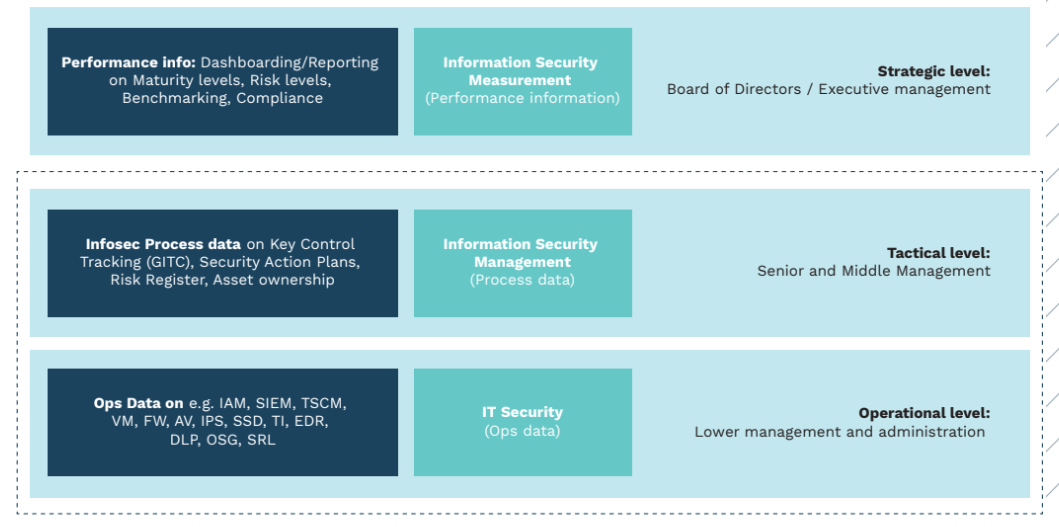
\includegraphics[scale=0.35]{Figures/stakeholders.png}}
    \caption{Cyber Security Stakeholders at Functional levels.}
    \label{fig:stakeholders}
\end{figure}
\FloatBarrier
The stakeholders
at a strategic level 
can be board of directors or an executive management, 
for example a Chief Information Security Officer (CISO) 
who is responsible for security related compliance 
and eventually also for its legal implications
\citep{farnham2013tools}. 
For a CISO, 
a cyber intelligence place them in an elevated knowledge zone 
of known risks 
and help to prepare their strategic decisions 
to tackle the potential risk,  
safeguarding and protecting the digital assets 
and safeguarding and protecting the business information. 

Tactical level stakeholders
transforms the strategic decisions to operational tasks 
and help Operational level to execute tasks 
for protection of digital assets and business information
\citep{farnham2013tools}.

\section{Problem Definition}

In this section, I have explicate the problem by first
explaining about the challenges being faced by the stakeholders in detail and then the over all implication of the problem on the stakeholder’s organisations. 
And lastly the impact if it does not get addressed.

\subsection{Problem}

The current status quo 
is that cyber news or cyber information 
are being pushed via multiple media 
\enquote{RSS, mail, WWW, news feeds etc} 
to multiple stakeholders of an organisation  
in a scattered way 
\citep{schales2011stream}
and are manually interpreted (see FIGURE \ref{fig:problem2}), 
this causes a dilute and incomplete picture 
\citep{liao2016acing}. 
Especially in a world where threats emerge 
in numbers and sophistication. 
In 2018 there where one billion unique malware samples counted
\citep{kucuk2020deceiving}.

\begin{figure}[ht]
    \centering
    \fbox{
\includegraphics[width=0.4\linewidth]{Figures/problem2.png}}
    \caption{Problem with information from multiple feeds. }
    \label{fig:problem2}
\end{figure}

\subsubsection{Impacted Stakeholder}

Stakeholders at every level faces problems 
with respect to cyber information and cyber intelligence
\citep{tounsi2018survey}. 
Stakeholders misses the fine link 
between cyber information and cyber intelligence 
due to volumetric issues, 
due to lack of contextualisation, 
due to lack of insight, 
due to lack of clear language and 
due to lack of advice \citep{barnum2012standardizing}.
Stakeholders concerns at each level are discussed below.

\subsubsection{Concerns at Strategic Levels}

The essence is to be aware of the latest news on cyber crimes 
and security breaches 
which can have legal implications. 
Here they face the problem of the need to scan 
the cyber newsfeed over thousand of intel sources 
before they can transform any cyber information into cyber intelligence.

\subsubsection{Concerns at Tactical Levels}

Their focus is to define the security action plans 
for the digital assets they hold the accountability. 
Here they have the problem to find the cyber information 
which is relevant to their digital assets and lack of advice. 

\subsubsection{Concerns at Operational Levels}

Their focus is to protect IT systems 
by taking required actions against the known threats 
and vulnerabilities 
defined in the security action plans; provided by the tactical level. 
Here they have the problem of time consumption 
for identifying systems, IOCs and solution analysis.

\begin{figure}
\centering
    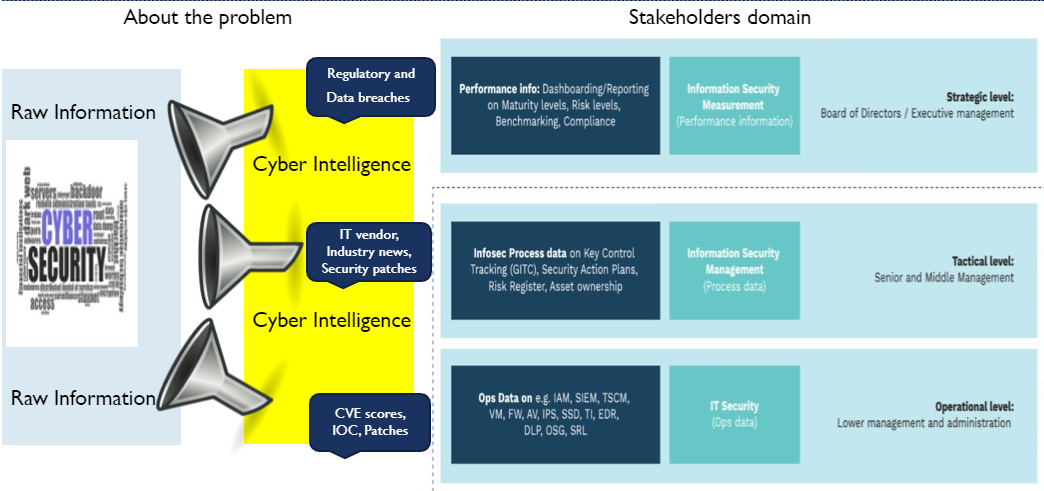
\includegraphics[scale=0.60]{Figures/stakeholder-problem.png}
    \caption{Stakeholders concerns at respective levels.}
    \label{fig:stakeholder-problem-domain}
\end{figure}


\subsection{Problem Statement}

There are Paid Sources and Open Sources to collect cyber information or cyber newsfeed into cyber intelligence platform- ‘Cyber-All-Intel’. ‘Cyber-All-Intel’ takes as input cybersecurity related text data from various unstructured sources like Dark Web, blogs, social media, National Vulnerability Databases (NVDs), newspaper articles, etc \citep{mittal2019cyber}. Other similar tools like 
Taranis\footnote{About Taranis \url{https://github.com/NCSC-NL/taranis3/wiki}}, 
IntelMQ\footnote{About IntelMQ \url{https://github.com/certtools/intelmq}}
and 
C1fApp\footnote{About C1fApp \url{https://www.c1fapp.com/}} 
are designed to collect, process and extract threat intelligence from open sources to obtain actionable cybersecurity information for the security analyst and advisors. 

\bigbreak

\textit{\textbf{But these tools require certain automations and efficient algorithms to filter, co-relate and tagging logics to make relevant cyber newsfeeds which get collected from over thousand of newsfeeds sources. 
And, it is difficult for stakeholders to manage enormous sources and exponentially available cyber information manually. 
This ultimately impacts the pace required to keep up to date with the Cyber threat Intelligence. 
Scanning all threats from all sources is tedious 
\citep{ghazi2018supervised} and most important is to transform and customize news feeds to make relevant for an organization in a specific sector, so that it could be operational and useful.
}
}

%----------------copy from res %question-------------------------------%-----------------------------------------------
\section{Research Question}\label{Research Question}
The scenario here is to transform the retrieved cyber threat information from multiple sources into organisation-specific cyber newsfeed intelligence. Would it be beneficial for the stakeholders if,  we could design a prototype artefact 1) to filter the cyber newsfeed into a specific context, 2) to tag relatable cyber newsfeeds data, and 3) to overcome the volumetric problem of sources for transforming cyber newsfeed into cyber intelligence?

As an example; given any vital sector
\citep[table 2]{luiijf2003critical} like water, housing, finance and hospitals, the companies who are subjective to EU directives\footnote{Directive (EU) 2016/1148 of the European Parliament and of the Council of 6 July 2016 concerning measures for a high common level of security of network and information systems across the Union: \url{http://data.europa.eu/eli/dir/2016/1148/oj}} would like to receive  cyber intelligence related to their digital landscape.

%\footnote{\url{https://en.wikipedia.org/wiki/Water_industry}}
\bigbreak
\textbf{How can we create a prototype, for filtering organisation-specific contextual cyber newsfeed, for tagging organisation-specific relatable cyber newsfeed, and for assessing the quality of the cyber newsfeed data sources; which can be validated by the stakeholders?}

\subsection{Sub-research questions}\label{Sub-research question}
To answer the aforementioned research question, we need to disseminate the research question into logical  sub-research questions to focus on granular details. With this problem  in mind, I  define three sub-research questions:

\begin{enumerate}
    \item What are elements in a cyber newsfeed processing chain and what are the parameters for automation?
    \begin{enumerate}
        \item What are the core concepts of cyber newsfeeds and how do they work according to the literature?
        
        \item How does the vendor field of automated cyber newsfeed suppliers of artefacts look like according to the literature?
    \end{enumerate}
    

    \item How to make a prototype to filter contextual cyber intelligence, perform automatic relevance tagging and perform analysis for risk determination and advisory?
    
    \item How to make a prototype for assessing the quality of the data sources?
    
    \item How to get the prototype validated for \emph{both 1) the design and 2) the output of this artefact} by the stakeholders of the specific organizations?
\end{enumerate}


\subsection{Research Deliverables}
An Implemented prototype artefact
for converting the cyber newsfeeds  
into relevant and contextual cyber intelligence 
based on  organisational-specific context 
and tags 
with results duly validated by the stakeholders.

\begin{enumerate}
   \item For Sub-research Question 1a and 1b: A literature review to explore the core concepts in the field of cyber newsfeed and   a literature review to explore the available artefacts.
       
  
    
    \item For Sub-research Question 2: 
    \begin{itemize}
        \item  A prototype which will have modules or sub-modules for collection, processing, analysis, publication and collection of user feedback. This is in chapter \ref{Chapter8_artefact-design}, section \label{New artefact prototype}, \nameref{New artefact prototype}.
        \item Power point presentation to the Cyber Analysts. Presentation listed in appendix \ref{Presentation to on2it}.
        \item Tool demonstration to the Cyber Analysts. It is in Chapter \ref{Chapter9_artefact-evaluation}, \nameref{Chapter9_artefact-evaluation} in section \ref{Demo Link},  \nameref{Demo Link}.
        
    \end{itemize}
    
   
     \item For Sub-research Question 3: A prototype to access the quality of data sources. This is presented in chapter \ref{Chapter8_artefact-design} section \ref{quality_source}, \nameref{quality_source}.
    \item For Sub-research Question 4:
    \begin{itemize}
    \item A demo of the simulated prototype and evaluation  report from the Focus group. Demo is in chapter  \ref{Chapter9_artefact-evaluation}, \nameref{Chapter9_artefact-evaluation} in section \ref{Demo Link} and evaluation report is in chapter \nameref{Chapter9_artefact-evaluation}, section \ref{Artefact Evaluation Results}, \nameref{Artefact Evaluation Results}. 
     \item Power point presentation to the Focus Group. Presentation listed in appendix  \ref{Presentation to GSS}.
        \item Tool demonstration to the Focus Group. It is in Chapter \ref{Chapter9_artefact-evaluation}, \nameref{Chapter9_artefact-evaluation} in section \ref{Demo Link},  \nameref{Demo Link}.
        \item Power point presentation to the CEO of a cybersecurity company. Presentation listed in appendix \ref{Presentation to CEO}.
       
     \end{itemize}
\end{enumerate}
The prototype was developed as a simulator software in coordination with ON2IT research department. An output of this simulation will be verified for the relevancy and actionability in the context of stakeholder’s interest.

\section{Conclusion}
With the end of this chapter, I have tried to help readers to get familiar with the problem background, and to understand the problem context; and expectations from this research work.








